\section{Finite excitation}

For the three values of $Q$ we now consider a situation with a finite excitation time such that $F(t) = F_0 \cos(\omega t)$ for $0 < t < T$ and $F(t) = 0$ for $t \geq T$. We can solve $x(t)$ analytically, using the result for a driving force of $F(t) = F_0 \cos(\omega t)$ for $t > 0$. Using this, we can find $x(T)$ and $\dot{x}(T)$. Subsequently, We can use this as the initial conditions in the same function $x(t)$, however with $F_0 = 0$. We also need to shift the function $t=T$ to future.

\begin{align*}
	x(t) = \begin{cases}
		x_1(t) & , \; 0 < t < T \\
		x_2(t-T) & , \; t \geq T \\
		\end{cases}
\end{align*}

With:

\begin{align*}
	x_1(t) = c_1 y_1(t) + c_2 y_2(t) + \frac{F_0 Q}{\omega^2 m}\sin(\omega t) \\
	x_2(t) = d_1 y_1(t) + d_2 y_2(t)
\end{align*}

$c_1$, $c_2$, $y_1$ and $y_2$ are defined as in the previous section and for $d_1$ and $d_2$:

\begin{align*}
	d_1 = \frac{1}{r_2-r_1} \left( -\dot{x}_1(T) + x_1(T) r_2 \right) \\
	d_2 = \frac{1}{r_2-r_1} \left( \dot{x}_1(T)  - x_1(T) r_1 \right) \\
\end{align*}

We can plot graphs for the values $\omega T = 0.1$, $\omega T = 1$ and $\omega T = 10$ for the three discussed values of $Q$. A scaled version of $F(t)$ is also plotted in the same axes in order to study the system with respect to the driving force:

\begin{figure}[h!]
	\centering
	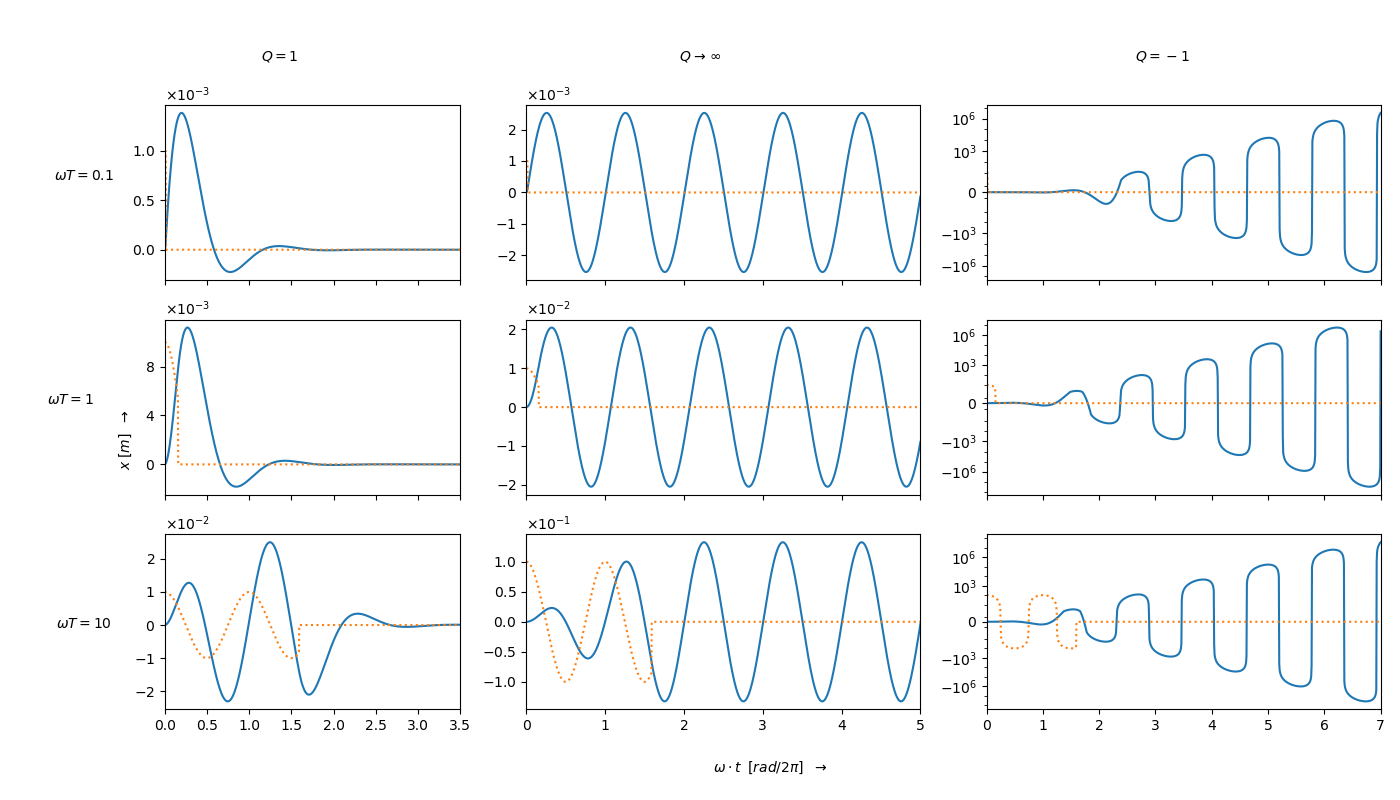
\includegraphics[width=0.8\textwidth]{figures/graph_q2.png}
	\caption{Graphs of $x(t)$ and $F(t)$  as function of $t$ for different values of $Q$ and $T$. The solid blue lines correspond with $x(t)$ and the orange dashed lines correspond to a scaled version of $F(t)$.}
	\label{fig_q1}
\end{figure}

We can make a number of observations from the graphs. Considering $Q = 1$, we find that , when there is no driving force, $x(t)$ will converge to zero. This is logical, since for $t>T$, there is only energy dissipation in the system by the friction. We also see that the graphs for $\omega T = 0.1$ and $\omega T =1$, the graphs are practically of identical shape, only differing by the amplitude and a slight time shift. The graph for $\omega T = 10$ shows that the shape of $x(t)$ is very different when $T$ is in a different phase of the oscillation.
For $Q \rightarrow \infty$ we find that for $t=T$, the oscillator will reach a steady state. This is logical since there is no energy dissipation or work done on the system. Therefore, the total energy in the system will remain constant. The amplitude of the steady state is the amplitude that corresponds with the energy in the system at $t=T$. We also see that the peaks of the three graphs are relatively close to each other. We can conclude from the graphs that the value of $T$ does not affect the shape of $x(t)$ and hardly affects the phase for an oscillator without friction. The amplitude is related to the excitation time.
For $Q=-1$ we see that the three graphs are very similar of shape, phase. Considering the logarithmic scale on the graphs, relative amplitude between $\omega T = 10$ and $\omega T = 0.1$ is more than a factor ten. The graphs do show some differences in shape in the long term. However, after about 2 oscillations, these differences become indiscernible. What's more is the amplification of the amplitude which seems equally for the three graphs and similar to the case with infinite excitation time in the previous section. It seems as for this system with 'inverse' friction. therefore, it seems as if the excitation time does not make a considerable difference to the system in the long term.\\


\section{Amplitude modulation}

We want to solve equation \ref{eq:to_solve} when a amplitude modulated external force is applied, this force follows from equation \ref{eq:force_q3}.\\

\begin{equation}
    m \ddot{x}(t)+m\frac{\omega}{Q}\dot{x}(t)+m \omega^2 x(t) = F(t)
    \label{eq:to_solve}
\end{equation}

\begin{equation}
    F(t) = F_0 t\frac{T-t}{T^2}= F_0 \frac{t}{T} - F_0 \frac{t^2}{T^2}
    \label{eq:force_q3}
\end{equation}

To solve equation \ref{eq:to_solve} numerically we first have to split the second order differential equations into a system of two first order equations. We do this by substituting two new time dependant functions for $y$, namely $u(t)$ and $v(t)$ equal to $y(t)$ and $y'(t)$ respectively. We can then derive the following system:\\

\begin{equation*}
    \left\{ \begin{matrix} \mbox{u(t) = y(t)}\\
    \mbox{v(t) = y'(t)} \end{matrix} \right.
\end{equation*}

So that their derivatives become:\\

\begin{equation*}
    \left\{ \begin{matrix} \mbox{u'(t) = y'(t) = v(t)}\\
    \mbox{v'(t) = y"(t)} \end{matrix} \right.
\end{equation*}

If we then substitute in these equations into the second order differential equation we get the following system:\\

\begin{align*}
    u'(t) &= y'(t) = v(t)\\
    v'(t) &= y''(t)\\
    F(t) &= m y''(t)+m\frac{\omega}{Q}y'(t)+m \omega^2 y(t)\\
\end{align*}

\begin{align*}
    v'(t) &= y''(t) = 1/m \cdot F(t) - \omega/Q\cdot y'(t)-\omega^2\cdot y(t)\\
    v'(t) &= 1/m\cdot F(t) - \omega/Q\cdot v(t)-\omega^2\cdot u(t)
\end{align*}

So that we now have the following system of of first-order linear differential equations:\\

\begin{align}
    v'(t) &= 1/m\cdot F(t)-\omega/Q\cdot v(t)- \omega^2\cdot u(t)\\
    u'(t) &= v(t)
\end{align}

This system can be easily solved numerically using the python code shown in the appendix section \ref{PythonCode}. We can then use a similar program to plot the nine different scenarios, these are shown in figure \ref{fig:fig_Q3}.\\

\vspace{-.5cm}
\begin{figure}[!h]
    \centering
    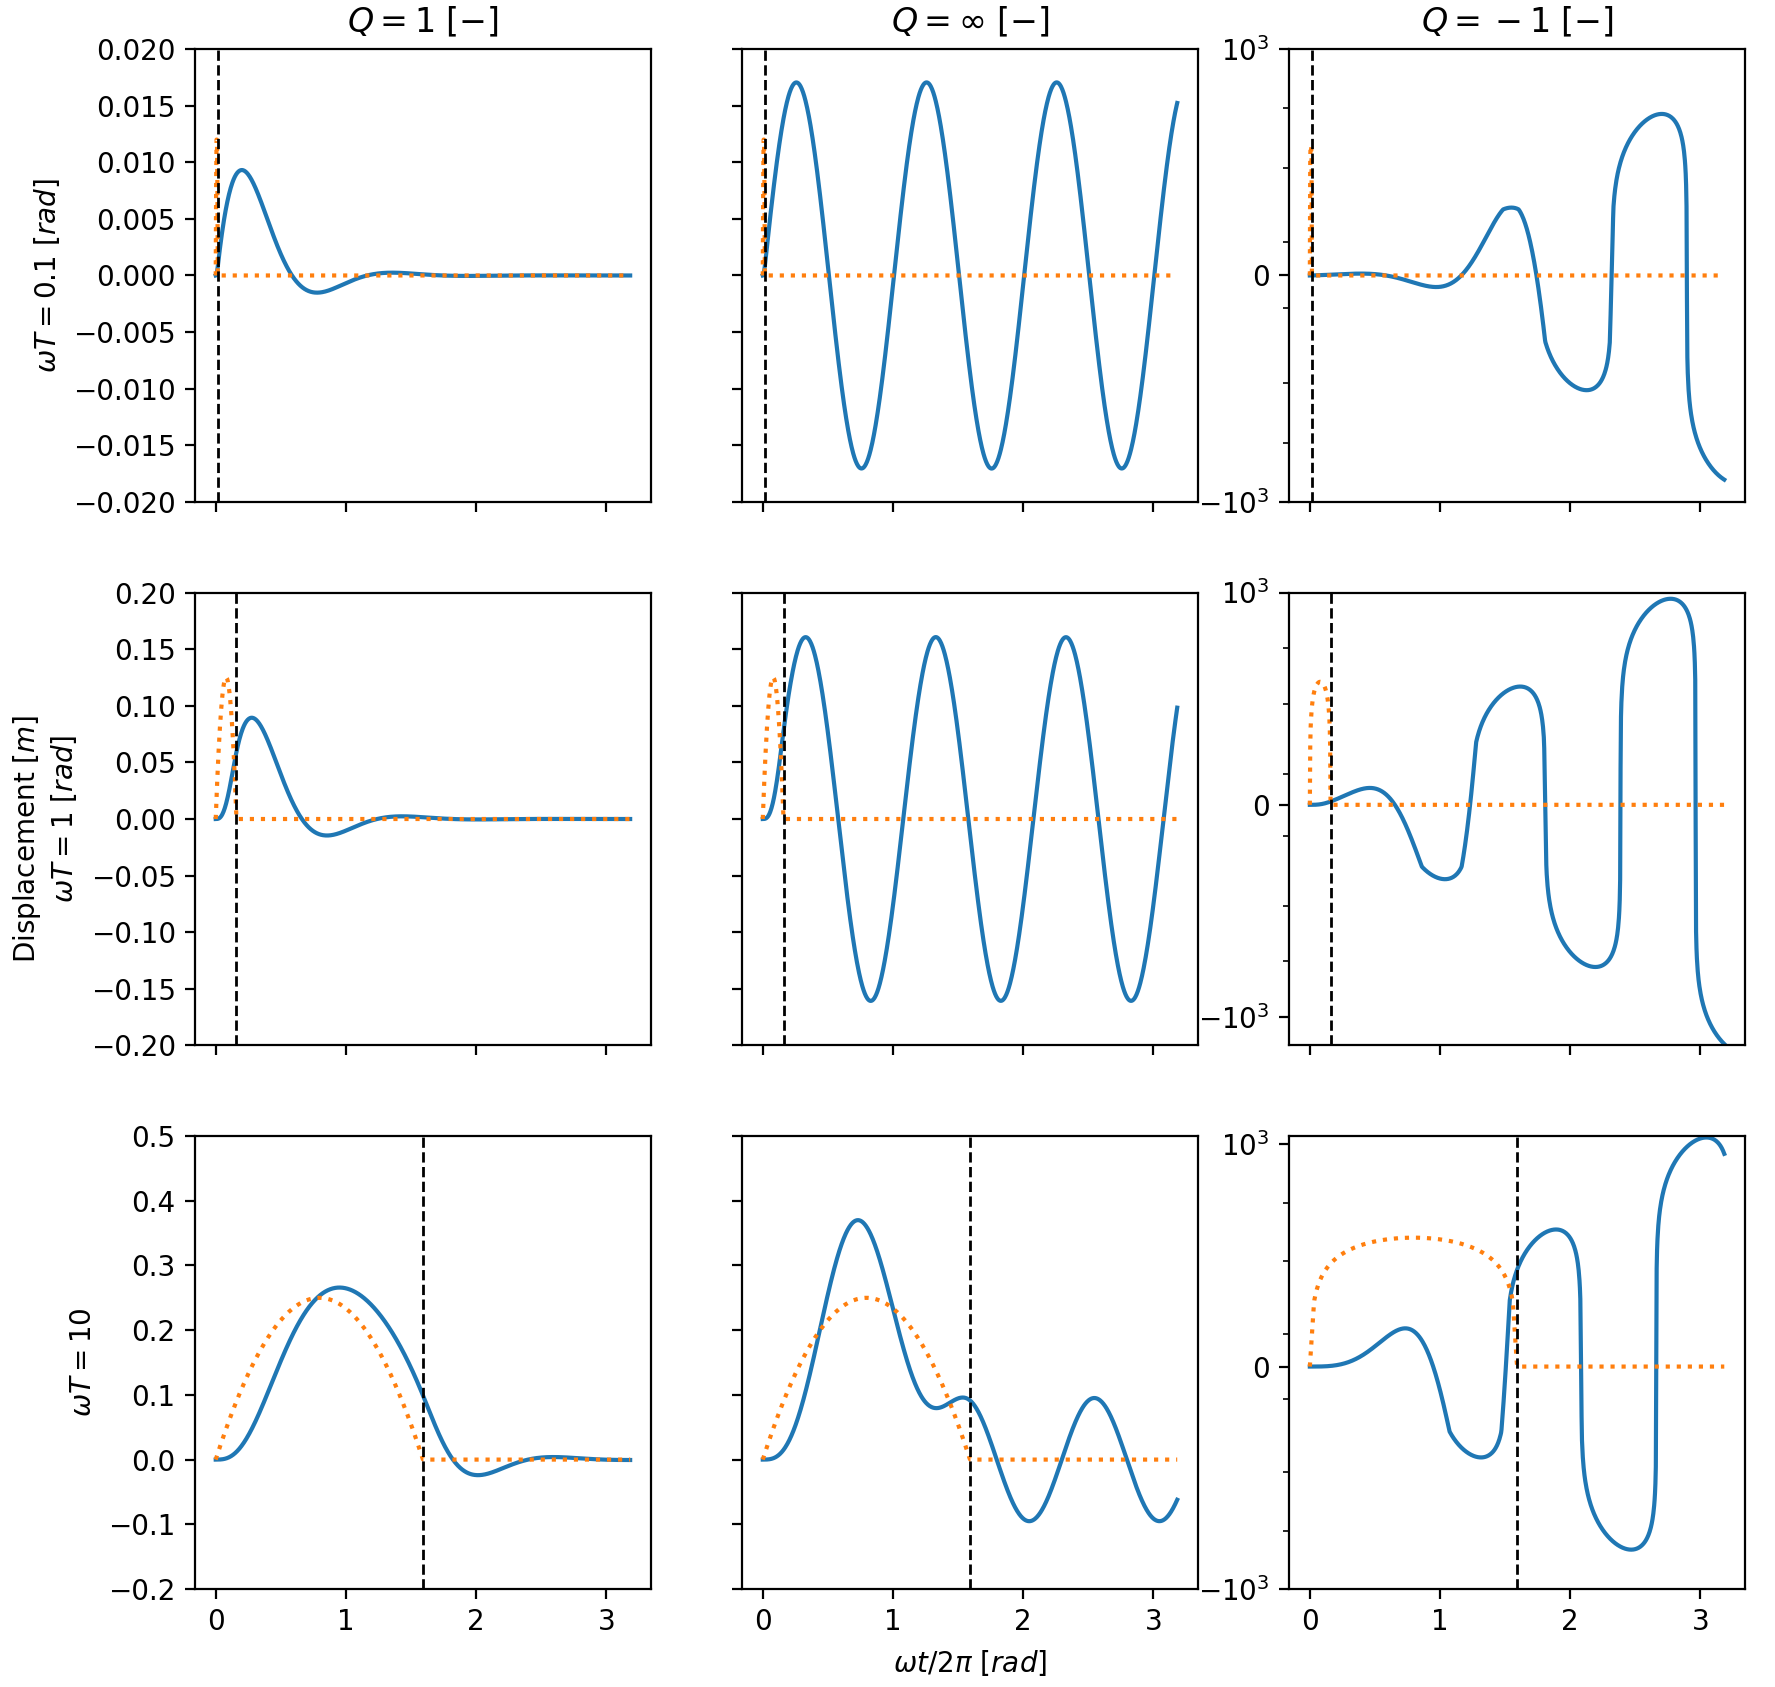
\includegraphics[width=.65\linewidth,keepaspectratio]{figures/Q3_omega_q_plot.png}
    \caption{The resulting oscillations for a parabolic force modulation. Here the displacement of the mass is plotted as a solid line and the force is plotted as the dashed line. The force is the same in all graphs but is scaled to emphasise the form. }
    \label{fig:fig_Q3}
\end{figure}

When looking at the graph we can see the different values of $\omega T$ plotted in rows and the different values of $Q$ in columns, all plots share the same time domain but only plots on the same row and in the first and second column share displacement axis.\\
The different values of $\omega T$ make noticeable differences in the graphs, the smallest value $\omega T = 0.1$ acts a lot like an impulse function, applying a short but strong force to set de oscillator into motion. We can see that for different quality factors the system reacts differently, for a normal friction force the system gradually returns to the equilibrium position, for $Q = \infty$ there is no friction force and the system start oscillating forever and looks like it had a starting velocity due to the short impulse force, for the quality factor of $Q = -1$ the friction force actually puts more energy into the system causing it to spiral out of control.
For the higher values of $\omega T$ we can see that the force is no longer representative of an impulse, meaning that the acceleration is not instantaneous, in the graph this can be seen by the small curve at the start of the plots where the oscillating mass needs to gain energy first. The different quality factors have the same effect as before.
The other noticeable effect is that in the bottom middle graph for $Q=\infty$ and $\omega T = 10$ we can see that the duration of the force applied is to long, at about 7 seconds the force starts to work against the oscillation thus having the adverse to the intended effect of a driving force. This effect can also be seen though less noticeably so with the graph to the left where the force is also pushing the mass away from equilibrium while the mass is already moving towards the equilibrium position.
It is clear from the plots that this type of modulation could alter the shape of the oscillation such that the motion only has only one broader pulse. This could possible be useful when sending data through oscillator modulation.\\